\documentclass[11pt,letterpaper,boxed]{hmcpset}
\usepackage{fullpage}
\setlength{\parskip}{6pt}
\setlength{\parindent}{0pt}
\usepackage[margin=1in]{geometry}
\usepackage{graphicx}
\usepackage{enumerate}
\usepackage{marvosym}
\usepackage{amssymb}
\usepackage{wasysym}
\usepackage{gensymb}
\usepackage{mathrsfs}
\usepackage{scrextend}
\usepackage{mathtools}
\usepackage{pgfplots}
\usepackage{xspace}
\usepackage[colorlinks]{hyperref}

\makeatletter
\renewcommand*\env@matrix[1][*\c@MaxMatrixCols c]{%
   \hskip -\arraycolsep
   \let\@ifnextchar\new@ifnextchar
   \array{#1}}
\makeatother

% --- style --- %
\renewcommand{\labelenumi}{{ (\alph{enumi})}}
\newcommand{\sand}{\quad \mbox{ and } \quad}
%\newcommand{\ds}{\displaystyle}
\allowdisplaybreaks

% --- making \xi look less awful --- %
\DeclareSymbolFont{CMletters}{OML}{cmm}{m}{it}
\DeclareMathSymbol{\xi}{\mathord}{CMletters}{"18}

% --- math --- %
\newcommand{\Z}{\mathbb{Z}}
\newcommand{\R}{\mathbb{R}}
\newcommand{\C}{\mathbb{C}}
\newcommand{\Q}{\mathbb{Q}}


\newcommand{\Lt}[1]{\mathcal{L}\crb{#1}}
\newcommand{\ilt}[1]{\mathcal{L}^{-1}\crb{#1}}

\newcommand{\pn}[1]{\left( #1 \right)}
\newcommand{\sqb}[1]{\left[ #1 \right]}
\newcommand{\crb}[1]{\left\{ #1 \right\}}
\newcommand{\lra}[1]{\left\langle #1 \right\rangle}
\newcommand{\magn}[1]{\left\lVert #1 \right\rVert}

\newcommand{\pdr}[2]{\frac{\partial #1}{\partial #2}}
\newcommand{\im}[1]{\text{im}\pn{#1}}
\newcommand{\m}[1]{\Z/#1\Z}

\newcommand{\VEC}[1]{\ensuremath{\mathbf{#1}}\xspace}
\DeclareMathOperator{\proj}{proj}
\newcommand{\vectorproj}[2][]{\proj_{\VEC{#1}}\VEC{#2}}

\newenvironment{amatrix}[1]{%
  \left(\begin{array}{@{}*{#1}{c}|c@{}}
}{%
  \end{array}\right)
}

\makeatletter
\renewcommand*\env@matrix[1][*\c@MaxMatrixCols c]{%
  \hskip -\arraycolsep
  \let\@ifnextchar\new@ifnextchar
  \array{#1}}
\makeatother

\newcommand{\spn}[1]{\text{span}\pn{#1}}

\newcommand*\Heq{\ensuremath{\overset{\kern2pt H}{=}}}

\name{Box \#$\rule{1cm}{0.15mm}$}
\class{Math 60 Section 1}
\assignment{Homework 11}
\duedate{30 May 2018}

\begin{document}

%\begin{center}
\noindent\textbf{Collaborators:} 
%\end{center} 

%\problemlist{}

\begin{problem}[Colley 6.2 \#13]
Evaluate $\oint_C \pn{x^4y^5-2y}dx + \pn{3x+x^5y^4}dy,$ where $C$ is the oriented curve pictured below
\begin{center}
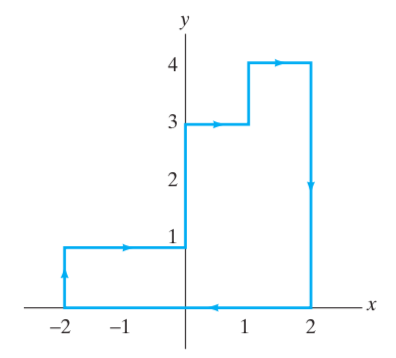
\includegraphics[scale=0.5]{fig1.png}
\end{center}
\end{problem}

\begin{solution}
\vfill
\end{solution}
\newpage

\begin{problem}[Colley 6.2 \#15]
\begin{enumerate}
\item Sketch the curve given parametrically by $\VEC{x}(t) = \pn{1-t^2, t^3-t}$.
\item Find the area inside the closed loop of the curve.
\end{enumerate}
\end{problem}

\begin{solution}
\vfill
\end{solution}
\newpage

\begin{problem}[Colley 6.3 \#1]
Consider the line integral $\int_C z^2\,dx+ 2y\,dy+ xz\,dz$.
\begin{enumerate}
\item Evaluate this integral, where $C$ is the line segment from $(0,0,0)$ to $(1,1,1)$.
\item Evaluate this integral, where $C$ is the path from $(0,0,0)$ to $(1,1,1)$ parametrized by $\VEC{x}(t) = (t,t^2,t^3), 0\leq t\leq1$.
\item Is the vector field $\VEC{F} = z^2\VEC{i} + 2y\VEC{j}+xz\VEC{k}$ conservative? Why or why not?
\end{enumerate}
\end{problem}

\begin{solution}
\vfill
\end{solution}
\newpage

\begin{problem}[Colley 6.3 \#3]
Determine whether the given vector field
\[
	\VEC{F} = e^{x+y}\VEC{i} + e^{xy}\VEC{j}
\]
is conservative. If it is, find a scalar potential function for $\VEC{F}$.
\end{problem}

\begin{solution}
\vfill
\end{solution}
\newpage

\begin{problem}[Colley 6.3 \#4]
Determine whether the given vector field
\[
	\VEC{F} = 2x\sin y\VEC{i} + x^2\cos y\VEC{j}
\]
is conservative. If it is, find a scalar potential function for $\VEC{F}$.
\end{problem}

\begin{solution}
\vfill
\end{solution}
\newpage

\begin{problem}[Colley 6.3 \#25]
Let $\VEC{F} = x^2\VEC{i} + \cos{y}\sin{z}	\VEC{j}+\sin{y}\cos{z}\VEC{k}$.
\begin{enumerate}
\item Show that $\VEC{F}$ is conservative and find a scalar potential function $f$ for $\VEC{F}$.
\item Evaluate $\int_{\VEC{x}}\VEC{F}\cdot d\VEC{s}$ along the path $\VEC{x}:[0,1]\rightarrow \R^3$, $\VEC{x}(t) = (t^2+1, e^t, e^{2t})$.
\end{enumerate}
\end{problem}

\begin{solution}
\vfill
\end{solution}
\newpage

\begin{problem}[Colley 6.3 \#33]
\begin{enumerate}
\item Determine whether the vector field
\[
	\VEC{F} = \frac{x+xy^2}{y^2}\VEC{i} - \frac{x^2+1}{y^3}\VEC{j}
\] 
is conservative.
\item Determine a scalar potential for $\VEC{F}$.
\item Find the work done by $\VEC{F}$ in moving a particle along the parabolic curve $y=1+x-x^2$ from $(0,1)$ to $(1,1)$.
\end{enumerate}
\end{problem}

\begin{solution}
\vfill
\end{solution}
\newpage

\begin{problem}[Colley 7.2 \#6]
Find $\int\int_S (x^2+y^2)\,dS$, where $S$ is the lateral surface of the cylinder of radius $a$ and height $h$ whose axis is the $z$-axis.	
\end{problem}

\begin{solution}
\vfill
\end{solution}
\newpage

\begin{problem}[Colley 7.2 \#14]
Let $S$ denote the closed cylinder with bottom given by $z=0$, top given by $z=4$, and lateral surface given by the equation $x^2+y^2=9$. Orient $S$ with
outward normals. Determine
\[
	\int\int_S \pn{x\VEC{i}+y\VEC{j}}\cdot d\VEC{S}.
\]
\end{problem}

\begin{solution}
\vfill
\end{solution}
\newpage

\begin{problem}[Colley 7.2 \#22]
Find the flux of
\[
	\VEC{F} = x^2\VEC{i} + xy\VEC{j}+xz\VEC{k}
\]
across the upper hemisphere $x^2+y^2+z^2=a^2$, $z\geq0$. Orient the hemisphere with an upward-pointing normal.
\end{problem}

\begin{solution}
\vfill
\end{solution}
\newpage

\begin{problem}[Colley 7.2 \#28]
The glass dome of a futuristic greenhouse is shaped like the surface $z=8-2x^2-2y^2$. The greenhouse has a flat dirt floor at $z = 0$. Suppose that the temperature $T$, at points in and around the greenhouse, varies as
\[
	T(x,y,z) = x^2+y^2+3(z-2)^2.
\]
Then the temperature gives rise to a \textbf{heat flux density field H} given by $\VEC{H} = -k\nabla T$. (Here $k$ is a positive constant that depends on the insulating properties of the particular medium.) Find the total heat flux outward across the dome and the surface of the ground if $k = 1$ on the glass and $k = 3$ on the ground.
\end{problem}

\begin{solution}
\vfill
\end{solution}
\newpage

\end{document}